\documentclass[11pt, a4paper]{article} % Font size
\usepackage[sfmath]{kpfonts}
\renewcommand*\familydefault{\sfdefault}

\usepackage{charter} % Use the Charter font for the document text
\usepackage[utf8]{inputenc}
\usepackage[T1]{fontenc}
\usepackage[spanish,es-nolayout,es-nodecimaldot,es-tabla]{babel}
\usepackage{amsmath}
\usepackage{amsfonts}
\usepackage{amssymb,amsthm}
\usepackage{enumerate}
\usepackage{enumitem}
\usepackage{parskip}
\usepackage{listings}
\usepackage{nicefrac}
\usepackage{framed, color}
\usepackage[left=2cm,right=2cm,top=2.5cm,bottom=2cm]{geometry}
\usepackage[colorlinks = true]{hyperref} 
\usepackage{wrapfig}
\usepackage[font={footnotesize,it}]{caption}
\usepackage{fancyhdr}
\pagestyle{fancy}
\usepackage{graphicx}
\renewcommand{\headrulewidth}{0pt}



\usepackage{lastpage}
\cfoot{\thepage\ de \pageref{LastPage}}

\makeatletter
\newcommand{\mathleft}{\@fleqntrue\@mathmargin0pt}
\newcommand{\mathcenter}{\@fleqnfalse}
\makeatother

\begin{document}\thispagestyle{empty}


\begin{flushleft}

\large
\rule{\textwidth}{1pt} \vspace{-1em} \par \noindent
\centerline{\LARGE			Recurso educativo		} 
\vspace{-0.75cm} \par\noindent%
\rule{\textwidth}{1pt} \par \noindent
%
%
\setlength{\tabcolsep}{0pt}%
%
\begin{tabular}{l@{\hspace{1em}}l}%
	\textbf{Editor:} 		& 	Antonio Merino\\ \\
	\textbf{Email:} 			& antonio23merino@hotmail.com\\
\end{tabular}%
\end{flushleft}
%
%
\rule{\textwidth}{1pt}  \vspace{-1em} \par \noindent
\centerline{\textbf{\Large		Variables aleatorias continuas		}} \vspace{-1em}
\par \noindent {\begin{center} \textit{Probabilidad y estadística} \end{center}} \vspace{-0.5em}
\rule{\textwidth}{1pt} \par \noindent


%%%%%%%%%%%%%%%%%%%

\textbf{Nota:} Lo siguiente, es un extracto del libro de probabilidad y estadística del Dr. Menthor Urvina


Intuitivamente podemos definir una variable aleatoria continua \(X\) sobre un espacio probabilístico \(\Omega\) como función

\begin{align}
	\begin{aligned}
	X : \quad &\Omega \to R \quad \text{tal que:} 
	\\ \nonumber
	 &P( \omega \, / \, X ( \omega ) = x ) = 0, \quad - \infty < x < \infty 
	 \\ \nonumber
	 &P(X = x) = 0 
	 \\ \nonumber
	\end{aligned}
\end{align}


\textbf{Definición.} Una variable aleatoria continua \(X\) sobre un espacio probabilístico \(\Omega\), es una función de valores reales tal que 
\(
\, \forall x \, \in \, \mathbb{R}, \{ \omega \, / \, X(\omega) = x \}
\) es vacío.

\textbf{Definición.} La función de distribución \(F\) de una variable aleatoria continua \(X\)  es la función definida por:

\(
F(x)=P(X \leq x)
\)

\textbf{Proposición.} Si \(X\) es una variable aleatoria continua, con \(F\) su función de distribución, se tiene:

\(
F(-\infty)=0; \quad	F(\infty)=1; \quad	0 \leq F(x) \leq 1\\
F
\) es contínua y no decreciente. 

\textbf{Definición.} Un función de densidad es una función no negativa, tal que:
\[
\int_{-\infty}^{\infty} f(x) \, dx=1
\]

\textbf{Nota.} si \(f\) es una función de densidad, entonces \(F\) definidad por

\[
F(x) \, = \, \int_{-\infty}^{x} f(y) \, dy
\]

Se llama la función de distribución.

Si \(X\) es una variable aleatoria continua que tiene a \(F\) como función de distribución, entonces:

\[
P(a \leq x \leq b) = F(b) - F(a)
\]

En general: 
\(
\, P(X \, \in \, A)= \, \int_{A} f(x) \, dx
\)

Así, 
\(
\, P(X \, \in \, A)
\)
puede ser interpretado como el área bajo la curva de \(f\) cuando \(x\) toma valores en \(A\)

\newpage

\begin{figure}[t!]
\centering
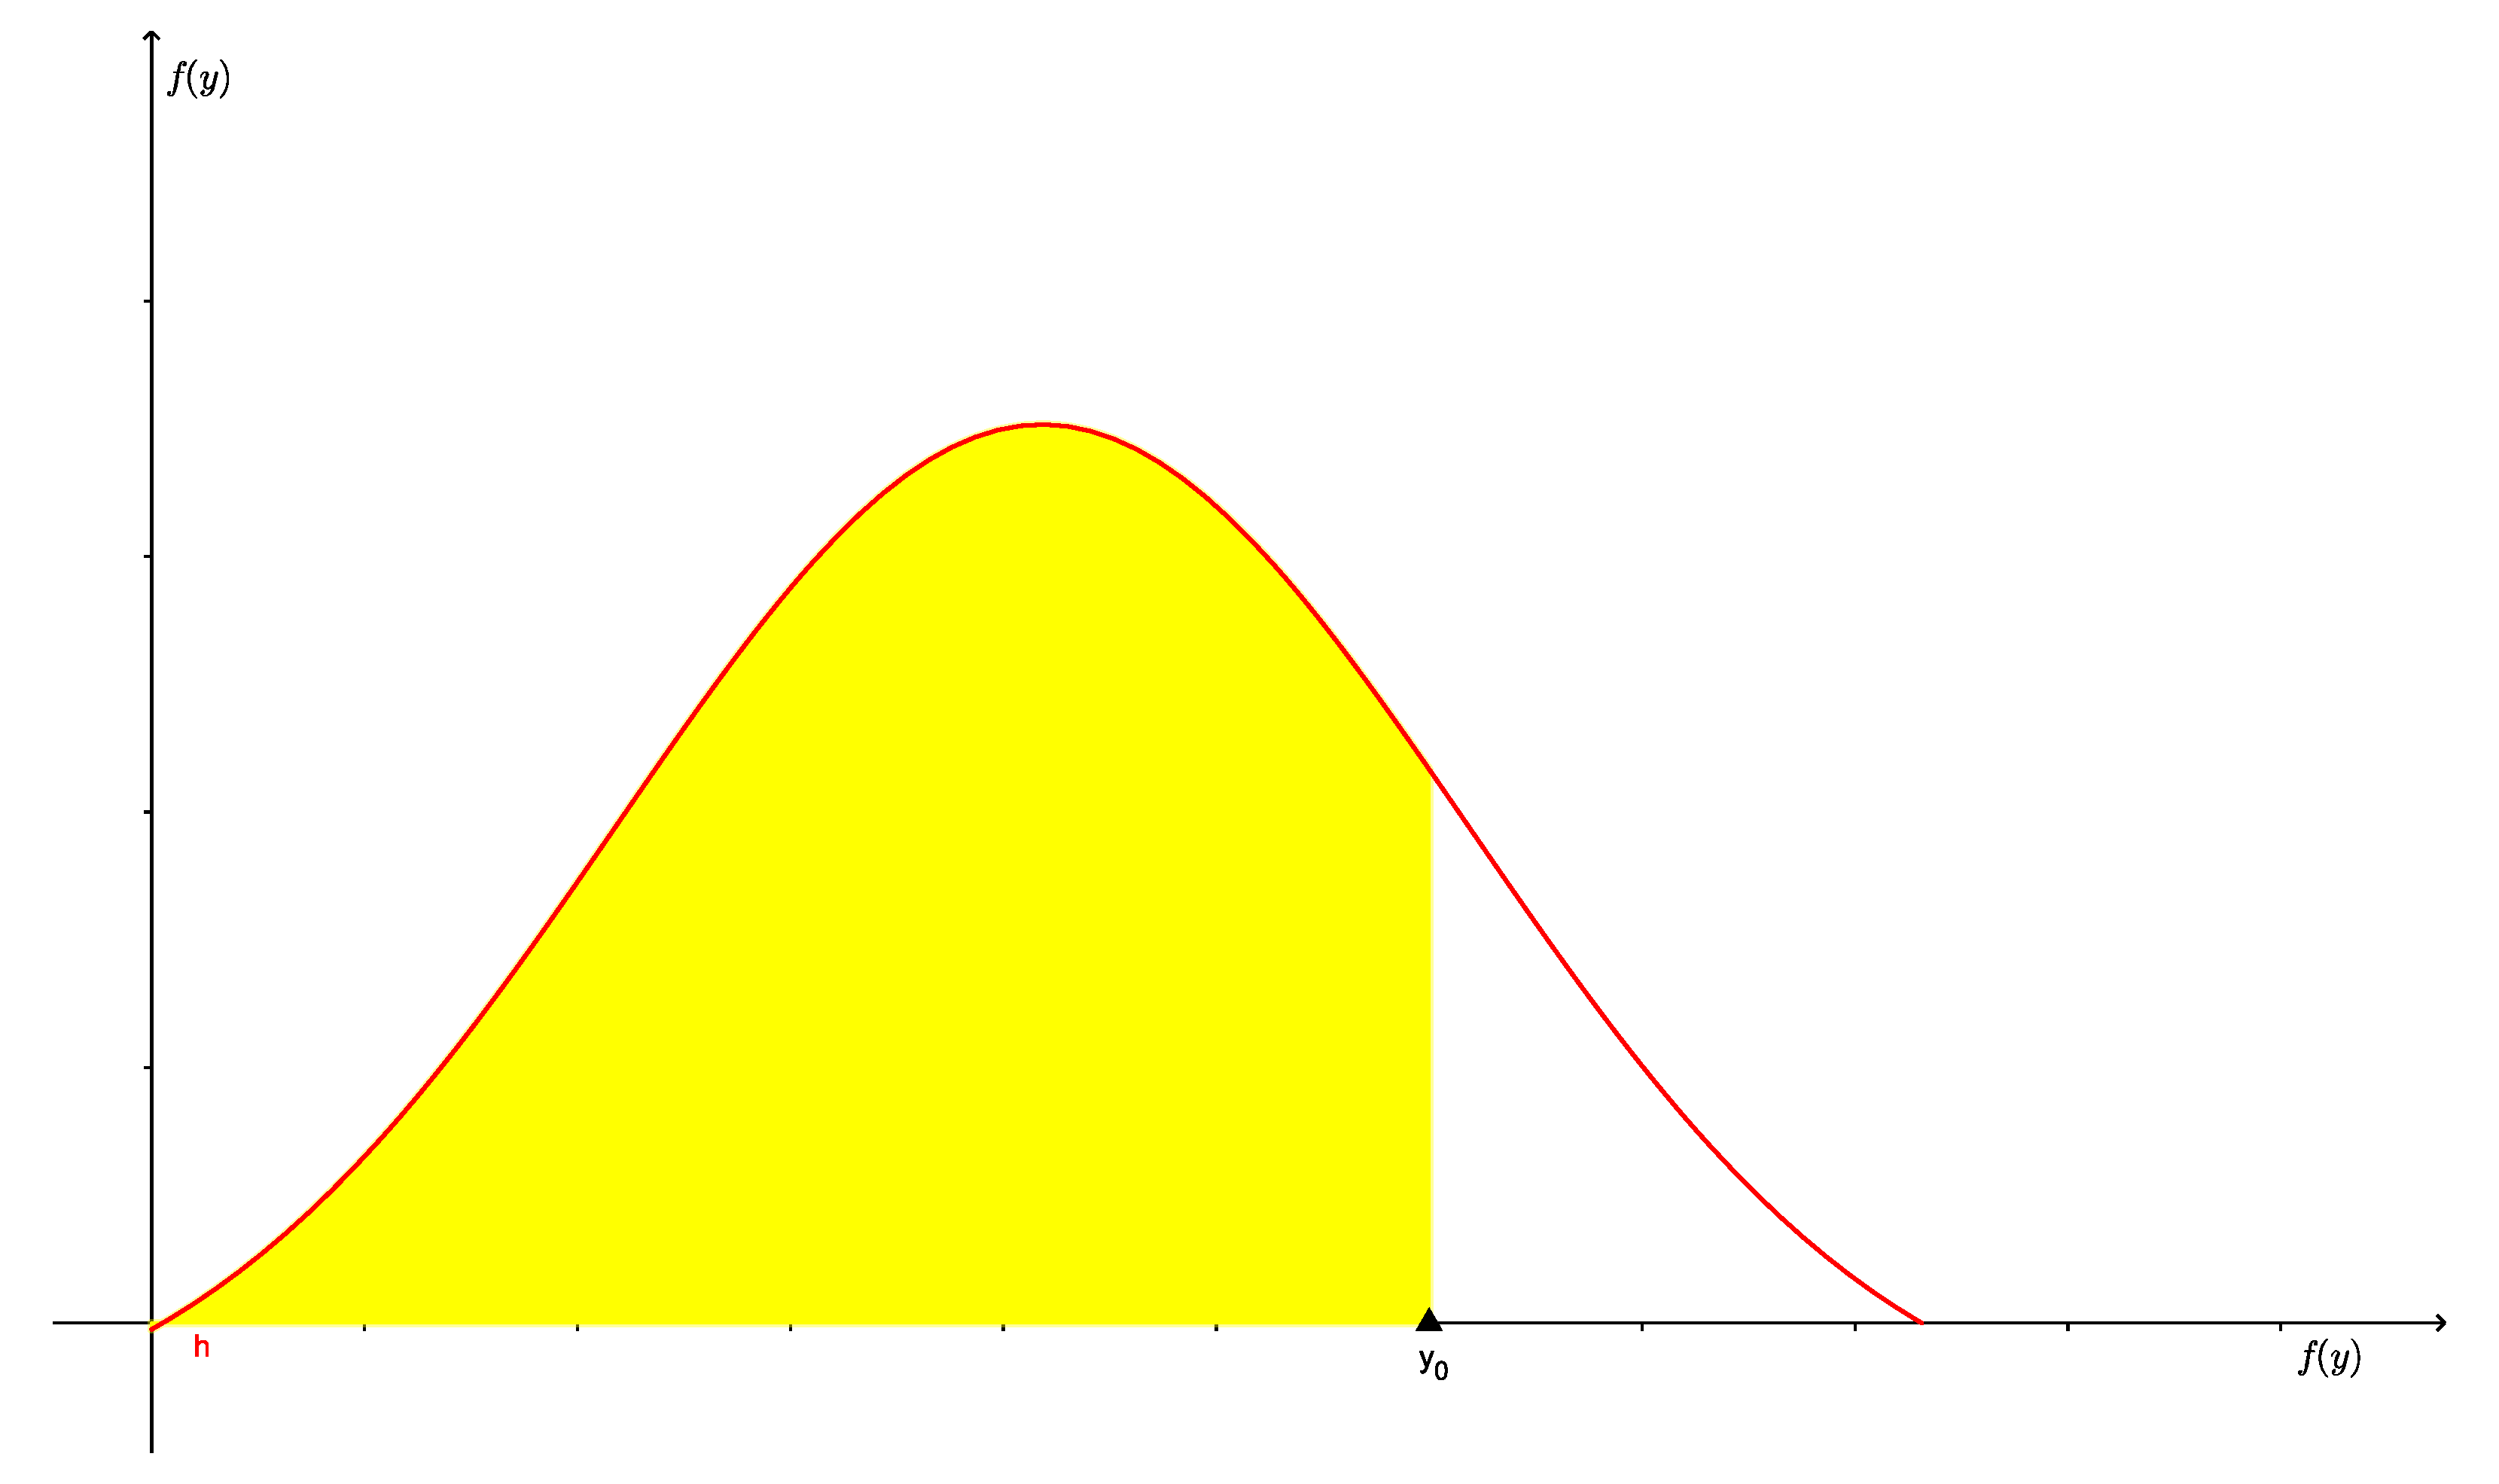
\includegraphics[scale=0.15]{distrnorm.pdf}
\end{figure}

\textbf{Observación.} En muchas aplicaciones el camino más fácil para hallar densidades de variables aleatorias es:

Si se conoce la función de distribución

\[
F(x)=P(X \leq x) \, = \, F(x) \,= \, \int_{-\infty}^{x} f(y) \, dy
\]

por el teorema fundamental del Cálculo se tiene: \, \(f(x) \, = \, F'(x)\)

lo cual se cumple \(\forall x \) donde \(f \) es continua

\textbf{Ejemplo.} La función de densidad de una variable aleatoria \(Z\) tiene la forma

\begin{align}
	f(z)
	=	
	\left\{ 
	\begin{aligned}
	&0, \qquad &z \quad < 1\\ \nonumber
	&z-1, \qquad 1\leq &z \quad \leq 2\\ \nonumber
	&3-z, \qquad 2\leq &z \quad \leq 3\\ \nonumber
	&0, \qquad &z \quad > 3\\ \nonumber
	\end{aligned}
	\right.
\end{align}

\begin{enumerate}[label=(\roman*)]
\item 
Hallar \(P(Z\leq \dfrac{3}{2})\); \, \(P(\dfrac{3}{2} \leq Z \leq \dfrac{5}{2})\); \, \(P(Z > \dfrac{5}{2})\)
\item
Hallar la función de distribución de \(Z\)
\end{enumerate}



\mathleft
\[
P(Z\leq \nicefrac{3}{2})
=
\, \int_{-\infty}^{\nicefrac{3}{2}} f(z) \, dz
=
\, \int_{-\infty}^{\nicefrac{3}{2}} (z-1) \, dz
=
\nicefrac{1}{8}
\\
\]

\[
P(\nicefrac{3}{2} \leq Z \leq \nicefrac{5}{2})
=
\, \int_{\nicefrac{3}{2}}^{2} (z-1) \, dz \, + \, \int_{2}^{\nicefrac{5}{2}} (3-z) \, dz  \, = \, \nicefrac{3}{4}
\\
\]

\[
P( Z > \nicefrac{5}{2})
=
\, \int_{\nicefrac{5}{2}}^{3} (3-z) \, dz \, = \, \nicefrac{1}{8}
\\
\]

\[
F(z)
=
\, \int_{-\infty}^{z} f(y) \, dy 
\\
\]

\begin{align}
\begin{aligned}
%%%
\text{si } z<1: \quad F(z)&=\, \int_{-\infty}^{z} f(y) \, dy = \, 0 
\\ \nonumber \\
%%%
1 \leq \, z<2: \quad F(z)&=\, \int_{-\infty}^{z} f(y) \, dy = 
\, \int_{1}^{z} f(y) \, dy \, = \, \int_{1}^{z} (y-1) \, dy = \, \dfrac{z^2}{2} - z + \dfrac{1}{2} 
\\ \nonumber \\
%%%
2 \leq z<3: \quad F(z)&=\, \int_{-\infty}^{z} f(y) \, dy = 
\, \int_{1}^{2} f(y) \, dy \, + \, \int_{2}^{z} (y-1) \, dy
\\ \nonumber \\
%%%
&=\, \int_{1}^{2} (y-1) \, dy \, + \, \int_{2}^{z} (3-y) \, dy = \quad \, 3z- \dfrac{z^2}{2} - \dfrac{7}{2}
\\
\end{aligned}
\end{align}

\textbf{Definición.} Sea \(X\) una variable aleatoria con función de densidad \(f\), se define la meadia o valor esperado de \(X\), que se denota por \(\mu_x\) o \(E[X]\), como

\mathcenter
\[
\mu_x = \int_{-\infty}^{\infty} xf(x) \, dx
\]

La viarianza de una variable aleatoria continua \(X\), que se denota por \(\sigma_x^2\) o \(Var[X]\), se define por:

\begin{align}
	\begin{aligned}	
		\sigma_x^2 \, &= \, E \big[ (X- \mu_x)^2 \big] \, = \, \int_{-\infty}^{\infty} (x- \mu_x)^2f(x) \, dx
		\\ \nonumber \\
		\sigma_x^2 \, &= \, E[(X)^2]- \big( E[X] \big)^2
		\\ \nonumber
	\end{aligned}
\end{align}

\textbf{Observación.} Si \(C\) es una constante,
\(
Y \, = \, X \, + \, C
\)

entonces:
\(
\sigma_Y^2 = \sigma_X^2 \, ; \quad \text{si } Y \, = \, CX \Rightarrow \quad \sigma_Y^2 = C^2\sigma_X^2
\)

\vspace{1\baselineskip}
\textbf{Ejemplo.} Para 
\(
f(x)=
	\left\{ \begin{aligned}
	0, \qquad &x<0\\ \nonumber
	2e^{-2x}, &x>0\\
	\end{aligned}
	\right.
\)

hallar la media y la varianza

\mathleft
\[
\mu \, = \, \int xf(x) \, dx \,
=
\, \int_0^\infty x.2e^{-2x} \, dx \,
=
\, \dfrac{1}{2}; \quad \sigma^2 \, 
=
\, \int_0^\infty \Big( x- \dfrac{1}{2} \Big)^2 f(x) \, dx \,
=
\, \dfrac{1}{4}
\]













\end{document}